\documentclass[11pt,fleqn]{article} 
\usepackage[margin=0.8in, head=0.8in]{geometry} 
\usepackage{amsmath, amssymb, amsthm}
\usepackage{fancyhdr} 
\usepackage{palatino, url, multicol}
\usepackage{graphicx} 
\usepackage[all]{xy}
\usepackage{polynom} 
\usepackage{pdfsync}
\usepackage{enumerate}
\usepackage{framed}
\usepackage{setspace, adjustbox}
\usepackage{array%,tikz, pgfplots
}

\usepackage{tikz, pgfplots}
\usetikzlibrary{calc}
%\pgfplotsset{my style/.append style={axis x line=middle, axis y line=
%middle, xlabel={$x$}, ylabel={$y$}, axis equal }}
%
\pagestyle{fancy} 
\lfoot{UAF Calculus I}
\rfoot{3-5 Implicit Differentiation}


\newcommand{\be}{\begin{enumerate}}
\newcommand{\ee}{\end{enumerate}}

\newcommand{\bi}{\begin{itemize}}
\newcommand{\ei}{\end{itemize}}

\begin{document}
\setlength{\parindent}{0cm}
\renewcommand{\headrulewidth}{0pt}
\newcommand{\blank}[1]{\rule{#1}{0.75pt}}
\renewcommand{\d}{\displaystyle}
\vspace*{-0.7in}
\begin{center}
 {\large{ \sc{Section 3.5 Implicit Differentiation}}}
\end{center}
\begin{enumerate}
\item Find $\frac{dy}{dx}$ for $2x+3y=xy-y^{2}$ and find the equations of tangents to the graph when $x=0.$ Use the graph below as an aid and to determine the plausibility of your answers.\\


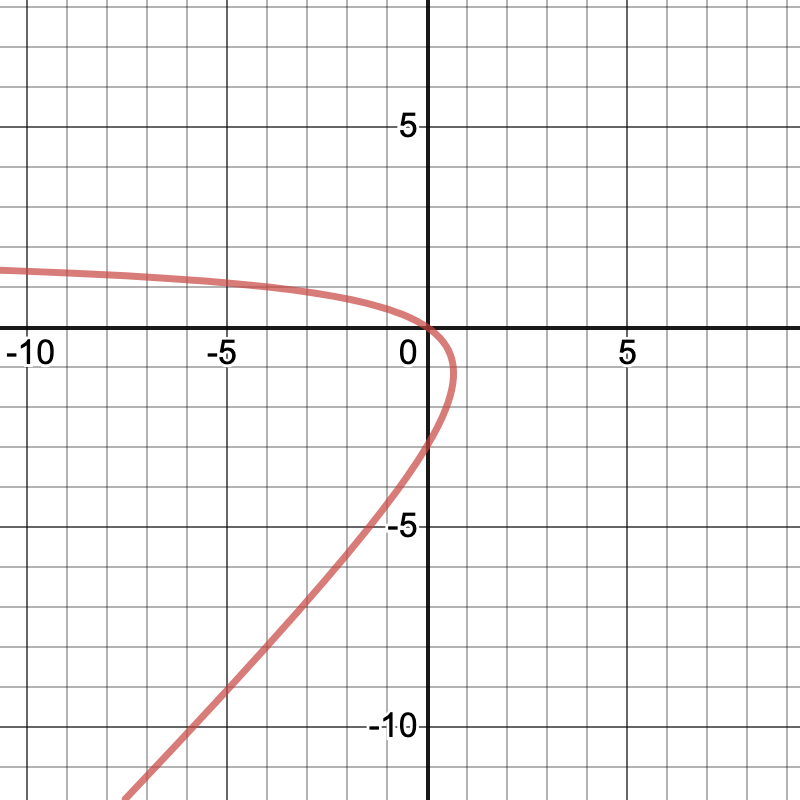
\includegraphics[scale=.25]{implicitgraph}

	
\item Find $\frac{da}{db}$ for $a^3\sin(3b)=a^2-b^2$
	\vfill
\item Find $\frac{dy}{dx}$ for $e^{xy}=x+y+1$
	\vfill

\newpage

\item You are going to derive the formula for the derivative of inverse tangent the way we found the derivative of inverse sine in class. 
	\begin{enumerate}
	\item Find $dy/dx$ for the expression $x=\tan(y).$
	\vfill
	\item Use the identity $1+\tan^2(\theta)=\sec^2(\theta)$ to rewrite you answer in part (a) and \emph{write your $dy/dx$ in terms of $x$ only}.
	\vfill
	\item Now fill in the blank $\d{\frac{d}{dx}\left[ \arctan(x)\right]}=$\\
	
	\item Use your knowledge of the \emph{graph} of $f(x)=\arctan(x)$ to decide if your answer seems plausible...
	\vspace{1in}
	\end{enumerate}
\item Find the derivative of $f(x)=x \arctan{x}.$
\vfill	

\item Find the derivative of $f(x) = \arctan ( 4-x^2).$
\vfill
\end{enumerate}
\end{document}